\documentclass[12pt, a4paper]{article}

% ── Encoding e lingua ──────────────────────────────────────────
\usepackage[T1]{fontenc}
\usepackage[utf8]{inputenc}
\usepackage[italian]{babel}

% ── Layout pagina ──────────────────────────────────────────────
\usepackage[top=2.5cm, bottom=2.5cm, left=2.8cm, right=2.8cm]{geometry}
\usepackage{setspace}
\onehalfspacing

% ── Font ───────────────────────────────────────────────────────
\usepackage{lmodern}
\usepackage{microtype}

% ── Colori e grafica ───────────────────────────────────────────
\usepackage[dvipsnames, table]{xcolor}
\definecolor{bluniapoli}{RGB}{0, 82, 147}
\definecolor{accento}{RGB}  {30, 120, 180}
\definecolor{sfondotab}{RGB}{235, 244, 252}
\definecolor{verdeat}  {RGB}{29, 158, 117}
\definecolor{rossoat}  {RGB}{226, 75, 74}
\definecolor{arancioat}{RGB}{186, 117, 23}

\usepackage{graphicx}
\graphicspath{{img/}}
\usepackage{float}
\usepackage{caption}
\captionsetup{font=small, labelfont=bf, labelsep=period}

% ── Tabelle ────────────────────────────────────────────────────
\usepackage{booktabs}
\usepackage{tabularx}
\usepackage{multirow}
\usepackage{array}

% ── Matematica ─────────────────────────────────────────────────
\usepackage{amsmath}
\usepackage{amssymb}

% ── Codice sorgente ────────────────────────────────────────────
\usepackage{listings}
\lstset{
  language=Python,
  basicstyle=\ttfamily\small,
  keywordstyle=\color{accento}\bfseries,
  commentstyle=\color{gray}\itshape,
  stringstyle=\color{verdeat},
  numberstyle=\tiny\color{gray},
  numbers=left,
  numbersep=8pt,
  breaklines=true,
  frame=single,
  framerule=0.4pt,
  rulecolor=\color{gray!40},
  backgroundcolor=\color{gray!5},
  xleftmargin=1.5em,
  xrightmargin=0.5em,
  showstringspaces=false,
  tabsize=4,
  captionpos=b,
}

% ── Hyperlink ──────────────────────────────────────────────────
\usepackage[hidelinks, colorlinks=true,
            linkcolor=accento, urlcolor=accento,
            citecolor=accento]{hyperref}

% ── Intestazioni sezione ───────────────────────────────────────
\usepackage{titlesec}
\titleformat{\section}
  {\large\bfseries\color{bluniapoli}}{\thesection.}{0.6em}{}[\color{bluniapoli}\titlerule]
\titleformat{\subsection}
  {\normalsize\bfseries\color{accento}}{\thesubsection.}{0.5em}{}
\titleformat{\subsubsection}
  {\normalsize\itshape\color{accento}}{\thesubsubsection.}{0.5em}{}

% ── Intestazione/piede pagina ──────────────────────────────────
\usepackage{fancyhdr}
\pagestyle{fancy}
\fancyhf{}
\fancyhead[L]{\small\textit{Elementi di Intelligenza Artificiale}}
\fancyhead[R]{\small\textit{Affari Tuoi e Machine Learning}}
\fancyfoot[C]{\thepage}
\renewcommand{\headrulewidth}{0.4pt}

% ── Caselle colorate ───────────────────────────────────────────
\usepackage{tcolorbox}
\tcbuselibrary{skins, breakable}
\newtcolorbox{riquadro}[2][]{
  colback=#2!6, colframe=#2!60!black,
  fonttitle=\bfseries\small, title=#1,
  boxrule=0.6pt, arc=4pt,
  left=6pt, right=6pt, top=4pt, bottom=4pt,
  #1
}

% ══════════════════════════════════════════════════════════════
\begin{document}
% ══════════════════════════════════════════════════════════════

% ── Frontespizio ───────────────────────────────────────────────
\begin{titlepage}
\centering
\vspace*{1.5cm}

{\Large\textbf{Università degli Studi di Napoli Federico II}}\par
\vspace{0.3cm}
{\large Dipartimento di Ingegneria Elettrica e delle Tecnologie dell'Informazione}\par
\vspace{0.2cm}
{\normalsize Corso di Laurea in Ingegneria Informatica}\par

\vspace{1.5cm}
\noindent\rule{\textwidth}{1.5pt}
\vspace{0.4cm}

{\LARGE\bfseries\color{bluniapoli}
Il Dottore sotto esame:\\ Machine Learning applicato alle offerte\\di \textit{Affari Tuoi}}\par

\vspace{0.4cm}
\noindent\rule{\textwidth}{1.5pt}

\vspace{1.2cm}
{\large Elaborato Finale}\par
\vspace{0.2cm}
{\normalsize Corso di \textbf{Elementi di Intelligenza Artificiale} 2025/2026}\par
\vspace{0.1cm}
{\normalsize Prof. Giancarlo Sperlì}\par

\vfill

\begin{tabular}{ll}
  \textbf{Studente:} &  Crisci Francesco Pio \\
  \textbf{Matricola:} & N46007601 \\
  \textbf{Studente:} & Raia Umberto \\
  \textbf{Matricola:} & N46007558 \\
\end{tabular}

\vspace{1cm}
 
\begin{center}
  {\small\texttt{\href{https://github.com/crrisci/dottore-affarituoi}{github.com/crrisci/dottore-affarituoi}}}
\end{center}

\vspace{1.5cm}
\end{titlepage}

% ── Indice ─────────────────────────────────────────────────────
\tableofcontents
\thispagestyle{empty}
\newpage
\setcounter{page}{1}

% ══════════════════════════════════════════════════════════════
\section{Introduzione}
% ══════════════════════════════════════════════════════════════

\textit{Affari Tuoi} è il programma televisivo più visto d'Italia nel 2024:
ogni sera oltre sei milioni di spettatori seguono un concorrente alle prese con
ventuno pacchi, ciascuno contenente un premio in denaro che va da 0~€ a 300.000~€.
Al centro dello show, letteralmente e metaforicamente, c'è il \textbf{Dottore}: un
personaggio misterioso che, a intervalli regolari, telefona per proporre al concorrente
una somma di denaro in cambio della rinuncia al proprio pacco.

Il programma ha scatenato negli ultimi mesi un acceso dibattito pubblico.
Matematici, statistici e appassionati si interrogano su una domanda fondamentale:
\textbf{le offerte del Dottore sono eque?} Oppure il Dottore calibra
strategicamente le sue proposte per minimizzare i pagamenti da parte della
produzione, sfruttando la pressione psicologica del momento?

L'obiettivo di questo progetto è rispondere a questa domanda con gli strumenti
dell'\textbf{intelligenza artificiale}, in particolare con il \textbf{Machine
Learning supervisionato}. A partire da un dataset di 89~puntate reali della
stagione 2023/2024, si è addestrato un sistema di classificazione in grado di
predire, dato lo stato della partita, se l'offerta del Dottore sarà
\textit{bassa}, \textit{media} o \textit{alta} rispetto al valore
statisticamente atteso. Le predizioni permettono poi di stimare, in termini
concreti, quanto il Dottore stia trattenendo rispetto a ciò che la matematica
suggerirebbe.

Il progetto è stato sviluppato interamente in \textbf{Python} con la libreria
\textit{scikit-learn}, con una replica del modello principale in
\textbf{KNIME Analytics Platform}.

% ══════════════════════════════════════════════════════════════
\section{Il Machine Learning}
% ══════════════════════════════════════════════════════════════

Il \textbf{Machine Learning} (ML) è una branca dell'Intelligenza Artificiale
che studia algoritmi e tecniche capaci di \emph{imparare dai dati}, migliorando
le proprie prestazioni attraverso l'esperienza senza essere esplicitamente
programmati per ogni caso specifico~\cite{mitchell1997}.

\subsection{Tipologie di apprendimento}

Esistono tre paradigmi principali:

\begin{itemize}
  \item \textbf{Apprendimento supervisionato}: il modello viene addestrato su un
        insieme di esempi etichettati, ossia coppie input--output già note.
        L'obiettivo è generalizzare la relazione appresa per predire l'output
        di nuovi dati. Questo progetto rientra in questa categoria.
  \item \textbf{Apprendimento non supervisionato}: il modello lavora su dati
        privi di etichette, cercando strutture e pattern nascosti
        (es.\ clustering, riduzione della dimensionalità).
  \item \textbf{Apprendimento per rinforzo}: un agente impara a prendere
        decisioni sequenziali interagendo con un ambiente, ricevendo ricompense
        o penalità in base alle azioni compiute.
\end{itemize}

\subsection{Classificazione e regressione}

Nell'apprendimento supervisionato si distinguono due tipi di problemi:

\begin{itemize}
  \item \textbf{Regressione}: la variabile target è continua
        (es.\ prevedere l'esatto importo dell'offerta in~€).
  \item \textbf{Classificazione}: la variabile target è categorica, cioè
        appartiene a un insieme finito di classi
        (es.\ classificare l'offerta come \textit{Bassa}, \textit{Media} o
        \textit{Alta}).
\end{itemize}

Per questo progetto si è scelto l'approccio della \textbf{classificazione a tre
classi}: la discretizzazione del problema lo rende più robusto alla varianza del
dataset (relativamente piccolo) e i risultati sono più facilmente interpretabili
e comunicabili.

\subsection{Le fasi del processo ML}

Un progetto di Machine Learning si articola in fasi ben definite, che
ricalcano quelle seguite in questo lavoro:

\begin{enumerate}
  \item \textbf{Raccolta e comprensione dei dati}: analisi esplorativa,
        identificazione delle feature rilevanti.
  \item \textbf{Pre-processing}: pulizia dei dati, gestione dei valori mancanti,
        normalizzazione, costruzione della variabile target.
  \item \textbf{Suddivisione train/test}: separazione dei dati in un insieme di
        addestramento e uno di valutazione, per stimare le prestazioni del
        modello su dati mai visti.
  \item \textbf{Addestramento}: il modello apprende i parametri ottimali
        minimizzando una funzione di errore sul training set.
  \item \textbf{Validazione}: la cross-validation stima la capacità di
        generalizzazione del modello.
  \item \textbf{Valutazione}: misurazione delle prestazioni sul test set tramite
        metriche standard (accuracy, precision, recall, F1-score).
\end{enumerate}

% ══════════════════════════════════════════════════════════════
\section{Il Dataset}
% ══════════════════════════════════════════════════════════════

\subsection{Fonte e raccolta dei dati}

I dati utilizzati provengono dal repository open-source
\href{https://github.com/luzo7/affari-tuoi}{\texttt{github.com/luzo7/affari-tuoi}},
realizzato da un appassionato del programma che ha sviluppato un software
specifico per registrare manualmente, puntata per puntata, ogni azione di gioco.
Il dataset copre un arco temporale di circa tre mesi e mezzo,
con puntate dal \textbf{12~febbraio~2024} al \textbf{20~maggio~2024}.

I dati grezzi sono memorizzati in formato \texttt{JSON} e descrivono la sequenza
completa di eventi di ogni partita: aperture di pacchi, offerte del Dottore,
accettazioni/rifiuti e tipo di fine partita.

\subsection{Struttura e statistiche descrittive}

\begin{table}[H]
\centering
\caption{Statistiche descrittive del dataset}
\rowcolors{2}{sfondotab}{white}
\begin{tabularx}{\textwidth}{lX}
  \toprule
  \textbf{Attributo} & \textbf{Valore} \\
  \midrule
  Numero di puntate         & 89 \\
  Totale offerte del Dottore & 386 \\
  Offerte accettate          & 41 (10,6\%) \\
  Offerte rifiutate          & 342 (88,6\%) \\
  Media valore offerta        & 30.770~€ \\
  Media valore atteso         & 41.007~€ \\
  Ratio medio offerta/VA      & 0,789 \\
  Ratio minimo                & 0,351 \\
  Ratio massimo               & 1,488 \\
  \bottomrule
\end{tabularx}
\label{tab:statistiche}
\end{table}

Il \textbf{ratio offerta/valore~atteso} è la metrica centrale del progetto.
È definito come:
\begin{equation}
  \text{ratio} = \frac{\text{offerta del Dottore}}{\mathbb{E}[\text{premi rimasti}]}
  = \frac{\text{offerta del Dottore}}{\frac{1}{n}\sum_{i=1}^{n} v_i}
  \label{eq:ratio}
\end{equation}
dove $n$ è il numero di pacchi ancora in gioco e $v_i$ è il valore del
pacco~$i$. Un ratio pari a~1 significa che il Dottore offre esattamente il
valore atteso matematico; valori inferiori indicano un'offerta penalizzante per
il concorrente.

I dati mostrano che in media il Dottore offre l'\textbf{78,9\%} del valore
atteso, trattenendo quindi circa il~21\% come ``margine''. Questo gap non è
uniforme nel corso della partita, come evidenziato nella Tabella~\ref{tab:turni}.

\begin{table}[H]
\centering
\caption{Comportamento del Dottore per turno di offerta}
\rowcolors{2}{sfondotab}{white}
\begin{tabular}{ccccc}
  \toprule
  \textbf{Turno} & \textbf{N.\ offerte} & \textbf{Ratio medio} & \textbf{Dev.\ std} & \textbf{Trattenuto medio (€)} \\
  \midrule
  1\textsuperscript{o} & 89 & 0,850 & 0,146 &  6.112 \\
  2\textsuperscript{o} & 86 & 0,751 & 0,153 & 11.113 \\
  3\textsuperscript{o} & 84 & 0,729 & 0,188 & 11.765 \\
  4\textsuperscript{o} & 67 & 0,776 & 0,199 & 12.218 \\
  5\textsuperscript{o} & 40 & 0,833 & 0,234 & 11.209 \\
  6\textsuperscript{o} & 16 & 0,894 & 0,324 &  9.879 \\
  7\textsuperscript{o} &  4 & 0,893 & 0,270 &  9.590 \\
  \bottomrule
\end{tabular}
\label{tab:turni}
\end{table}

Emerge un pattern inequivocabile: il Dottore è più generoso nella prima offerta
(ratio~0,850) per ``agganciare'' il concorrente, diventa più aggressivo al
terzo e quarto turno (ratio~0,729--0,776, quando la pressione psicologica è
massima e i pacchi ad alto valore sono ancora molti), per poi tornare a offrire
di più nelle fasi finali quando il numero di pacchi rimasti è ridotto.

\subsection{Analisi esplorativa}

I tipi di conclusione delle 89 puntate sono distribuiti come segue:
40 puntate si concludono con l'\textbf{accettazione di un'offerta} (44,9\%),
28 con l'\textbf{apertura del proprio pacco} (31,5\%) e 21 grazie alla
\textbf{Regione fortunata} (23,6\%).

\begin{figure}[H]
  \centering
  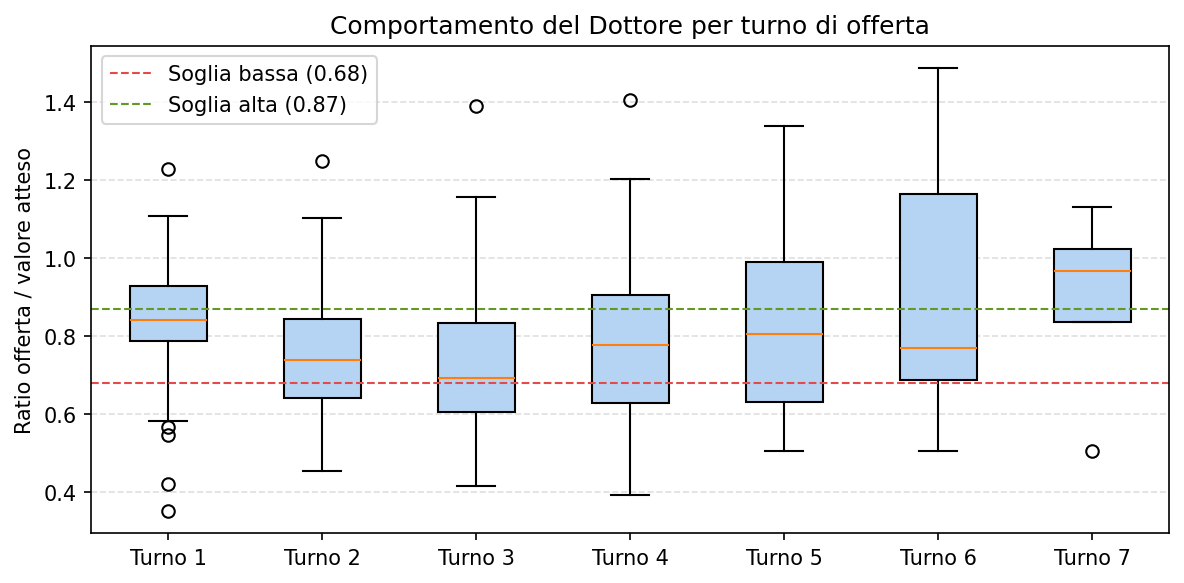
\includegraphics[width=0.95\textwidth]{ratio_per_turno.png}
  \caption{Distribuzione del ratio offerta/valore atteso per turno. Le linee
           tratteggiate indicano le soglie di classificazione: sotto 0,68 (rosso)
           l'offerta è classificata come \textit{Bassa}, sopra 0,87 (verde)
           come \textit{Alta}.}
  \label{fig:boxplot}
\end{figure}

\begin{figure}[H]
  \centering
  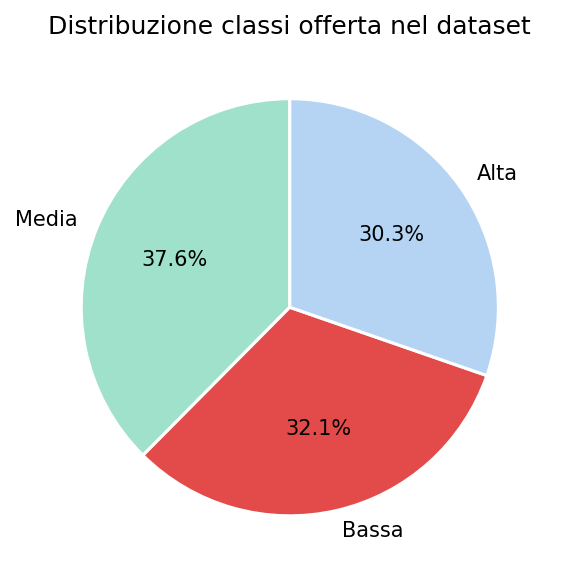
\includegraphics[width=0.48\textwidth]{distribuzione_classi.png}
  \caption{Distribuzione delle tre classi nel dataset (386 offerte totali).}
  \label{fig:torta}
\end{figure}

% ══════════════════════════════════════════════════════════════
\section{Feature Engineering e Pre-processing}
% ══════════════════════════════════════════════════════════════

\subsection{Estrazione delle feature}

A partire dal file JSON grezzo, si è ricostruito lo \textbf{stato della partita
in corrispondenza di ogni offerta}: per ogni azione di apertura si rimuove il
valore corrispondente dal pool dei 21 premi disponibili, aggiornando
dinamicamente le statistiche. Le feature calcolate per ciascuna delle 386
offerte sono riassunte nella Tabella~\ref{tab:feature}.

\begin{table}[H]
\centering
\caption{Feature di input utilizzate dai modelli}
\rowcolors{2}{sfondotab}{white}
\begin{tabular}{llp{6.5cm}}
  \toprule
  \textbf{Feature} & \textbf{Tipo} & \textbf{Descrizione} \\
  \midrule
  \texttt{num\_offerta}       & Intero  & Numero progressivo dell'offerta nella puntata (1--7) \\
  \texttt{n\_pacchi\_rimasti} & Intero  & Numero di pacchi ancora in gioco (3--15) \\
  \texttt{valore\_atteso}     & Float   & Media aritmetica dei premi rimasti (€) \\
  \texttt{mediana\_rimasti}   & Float   & Mediana dei premi rimasti, meno sensibile agli outlier \\
  \texttt{max\_rimasto}       & Intero  & Premio massimo ancora in gioco (€) \\
  \texttt{min\_rimasto}       & Intero  & Premio minimo ancora in gioco (€) \\
  \texttt{std\_rimasti}       & Float   & Deviazione standard dei premi rimasti \\
  \texttt{n\_valori\_alti}    & Intero  & Numero di pacchi con valore $\geq$~50.000~€ \\
  \bottomrule
\end{tabular}
\label{tab:feature}
\end{table}

Non sono stati rilevati \textbf{valori mancanti} nel dataset. Ogni offerta è
completamente descritta dalle otto feature sopra elencate.

\subsection{Costruzione della variabile target}

La variabile dipendente è il \textbf{tipo di offerta}, classificata in tre
categorie sulla base del ratio definito nella~\eqref{eq:ratio}.
Le soglie sono state calibrate sulla distribuzione empirica dei dati,
prendendo come riferimento i percentili~$P_{32}$ e $P_{70}$, in modo da
ottenere classi il più possibile bilanciate:

\begin{itemize}
  \item \textbf{Bassa} (classe~0): ratio $< 0{,}68$ \quad
        $\Rightarrow$ 124 offerte (32,1\%)
  \item \textbf{Media} (classe~1): $0{,}68 \leq$ ratio $\leq 0{,}87$ \quad
        $\Rightarrow$ 145 offerte (37,6\%)
  \item \textbf{Alta} (classe~2): ratio $> 0{,}87$ \quad
        $\Rightarrow$ 117 offerte (30,3\%)
\end{itemize}

\subsection{Normalizzazione e suddivisione del dataset}

Le feature numeriche sono state normalizzate tramite \textbf{MinMaxScaler},
che mappa ogni valore nell'intervallo $[0, 1]$:
\begin{equation}
  x' = \frac{x - x_{\min}}{x_{\max} - x_{\min}}
\end{equation}

La normalizzazione è inclusa all'interno delle pipeline di scikit-learn, in modo
da essere ricalcolata esclusivamente sui dati di addestramento in ogni fold della
cross-validation, \textbf{evitando il data leakage}.

Il dataset è stato suddiviso con proporzione \textbf{75\% train / 25\% test},
con stratificazione sulla variabile target per preservare la distribuzione delle
classi:
\begin{itemize}
  \item Training set: \textbf{289 campioni}
  \item Test set: \textbf{97 campioni}
\end{itemize}

% ══════════════════════════════════════════════════════════════
\section{Modelli di Classificazione}
% ══════════════════════════════════════════════════════════════

Sono stati addestrati e confrontati tre classificatori supervisionati,
scelti per la loro complementarietà teorica e per la loro rilevanza nel
contesto del corso.

\subsection{Decision Tree}

L'\textbf{albero decisionale} è un classificatore che costruisce un modello
a struttura gerarchica: ogni nodo interno rappresenta un test su una feature,
ogni ramo è l'esito del test, ogni foglia è una classe~\cite{breiman1984}.
La predizione si ottiene percorrendo l'albero dalla radice alla foglia.

Il criterio di split usato è la \textbf{Gini impurity}, che misura la probabilità
che un campione scelto casualmente venga classificato in modo errato:
\begin{equation}
  G = 1 - \sum_{k=1}^{K} p_k^2
\end{equation}
dove $p_k$ è la proporzione di campioni di classe~$k$ nel nodo.

Il parametro \texttt{max\_depth=5} limita la profondità dell'albero per
\textbf{prevenire l'overfitting}: senza tale vincolo, il Decision Tree tende
a memorizzare il training set senza generalizzare.

\subsection{Random Forest}

La \textbf{foresta casuale} è un metodo di \textit{ensemble learning} che
combina le predizioni di un numero elevato di alberi decisionali addestrati in
modo indipendente~\cite{breiman2001}. L'idea alla base è il principio
della \textbf{saggezza della folla}: modelli diversi commettono errori diversi,
e la loro aggregazione (per votazione a maggioranza nel caso della
classificazione) riduce significativamente la varianza.

La diversità tra gli alberi è garantita da due meccanismi:
\begin{enumerate}
  \item \textbf{Bagging} (\textit{Bootstrap Aggregating}): ogni albero è
        addestrato su un campione con ripetizione (\textit{bootstrap}) del
        training set.
  \item \textbf{Feature randomness}: ad ogni split, solo un sottoinsieme
        casuale di $\sqrt{p}$ feature viene considerato (con $p$ il numero
        totale di feature).
\end{enumerate}

Nel progetto si è usata una foresta di \texttt{n\_estimators=100} alberi.
La Random Forest fornisce inoltre la \textbf{feature importance}, una misura
di quanto ogni variabile contribuisce alla riduzione dell'impurità media
attraverso tutti gli alberi.

\subsection{Naive Bayes}

Il classificatore \textbf{Naive Bayes} sfrutta il teorema di Bayes per stimare
la probabilità a posteriori di ogni classe dato un vettore di feature:
\begin{equation}
  P(C_k \mid \mathbf{x}) = \frac{P(\mathbf{x} \mid C_k)\, P(C_k)}{P(\mathbf{x})}
\end{equation}

L'assunzione ``naive'' è la \textbf{indipendenza condizionale} tra le feature
dato la classe: $P(\mathbf{x} \mid C_k) = \prod_{j} P(x_j \mid C_k)$.
Nella variante \textbf{Gaussiana} adottata, si assume che ogni feature,
condizionatamente alla classe, segua una distribuzione normale:
$P(x_j \mid C_k) = \mathcal{N}(\mu_{jk}, \sigma_{jk}^2)$.

Nonostante la semplicità dell'assunzione (raramente soddisfatta in pratica),
Naive Bayes è noto per la sua robustezza e velocità di addestramento,
specialmente su dataset di dimensioni ridotte.

% ══════════════════════════════════════════════════════════════
\section{Implementazione}
% ══════════════════════════════════════════════════════════════

\subsection{Implementazione Python}

Il progetto è stato interamente implementato in \textbf{Python~3}, facendo uso
delle seguenti librerie principali:
\begin{itemize}
  \item \texttt{json}, \texttt{numpy}, \texttt{pandas}: lettura del dataset
        e manipolazione dei dati;
  \item \texttt{scikit-learn}: pre-processing, addestramento,
        cross-validation e metriche;
  \item \texttt{matplotlib}: generazione dei grafici.
\end{itemize}

L'architettura del codice segue il paradigma delle \textbf{pipeline} di
scikit-learn, che incapsulano in un unico oggetto la sequenza di trasformazioni
e il classificatore finale. Questo approccio garantisce l'assenza di data
leakage durante la cross-validation.

\begin{lstlisting}[caption={Definizione delle pipeline e cross-validation}, label={lst:pipeline}]
from sklearn.pipeline import make_pipeline
from sklearn.preprocessing import MinMaxScaler
from sklearn.tree import DecisionTreeClassifier
from sklearn.ensemble import RandomForestClassifier
from sklearn.naive_bayes import GaussianNB
from sklearn.model_selection import KFold, cross_val_score

# Ogni pipeline: normalizzazione + classificatore
pipelines = {
    "Decision Tree": make_pipeline(
        MinMaxScaler(),
        DecisionTreeClassifier(random_state=42, max_depth=5)
    ),
    "Random Forest": make_pipeline(
        MinMaxScaler(),
        RandomForestClassifier(n_estimators=100, random_state=42)
    ),
    "Naive Bayes": make_pipeline(
        MinMaxScaler(),
        GaussianNB()
    ),
}

# Cross-validation stratificata con 10 fold
kfold = KFold(n_splits=10, shuffle=True, random_state=42)

for nome, pipeline in pipelines.items():
    scores = cross_val_score(
        pipeline, X_train, y_train,
        cv=kfold, scoring="accuracy"
    )
    print(f"{nome}: media={scores.mean():.3f}, std={scores.std():.3f}")
\end{lstlisting}

\subsection{Implementazione KNIME}

La Random Forest è stata replicata in \textbf{KNIME Analytics Platform}
(versione~5), una piattaforma open-source per l'analisi visuale dei dati
basata su flussi di lavoro a nodi. L'implementazione KNIME ha lo scopo
principale di fornire una \textbf{rappresentazione grafica della pipeline},
particolarmente utile per comunicare il processo a un pubblico non tecnico,
e di verificare la correttezza logica della sequenza di operazioni.

Il workflow, mostrato in Figura~\ref{fig:knime_workflow}, comprende
i seguenti 7 nodi collegati in sequenza:

\begin{enumerate}
  \item \textbf{CSV Reader}: importazione del file \texttt{dataset\_offerte.csv}
        generato dallo script Python (386 righe, 12 colonne);
  \item \textbf{Column Filter}: selezione delle 8 feature di input
        e della colonna target \texttt{classe\_offerta};
  \item \textbf{Normalizer} (Min-Max): normalizzazione nell'intervallo $[0,1]$
        delle 8 feature numeriche, escludendo il target;
  \item \textbf{Row Sampler}: campionamento stratificato del 75\% dei dati
        per il training (seed~42);
  \item \textbf{Random Forest Learner}: addestramento del modello con
        100 alberi, colonna target \texttt{classe\_offerta};
  \item \textbf{Random Forest Predictor}: applicazione del modello addestrato
        ai dati in ingresso;
  \item \textbf{Scorer}: calcolo della matrice di confusione e delle
        statistiche di classificazione.
\end{enumerate}

\begin{figure}[H]
  \centering
  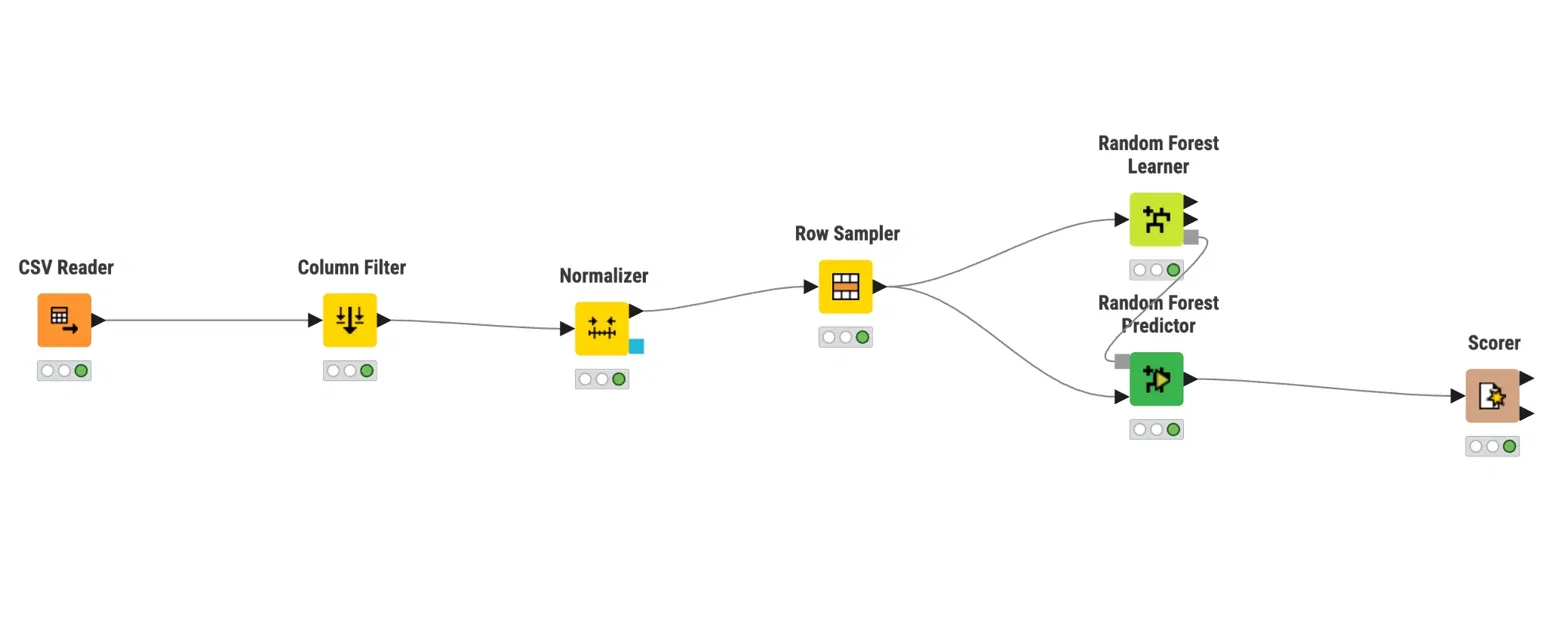
\includegraphics[width=\textwidth]{knime_workflow.png}
  \caption{Workflow KNIME 5 per la classificazione delle offerte del Dottore.
           Da sinistra: CSV Reader $\to$ Column Filter $\to$ Normalizer $\to$
           Row Sampler $\to$ Random Forest Learner / Predictor $\to$ Scorer.}
  \label{fig:knime_workflow}
\end{figure}

\paragraph{Nota sul confronto con Python.}
A differenza dell'implementazione Python, in KNIME~5 il nodo
\textit{Row Sampler} dispone di una sola porta di uscita: produce il
75\% dei dati destinato al training, ma non espone separatamente il
restante 25\% come test set indipendente. Di conseguenza, il Predictor
valuta lo stesso insieme su cui il Learner è stato addestrato, producendo
un'accuracy artificialmente elevata (99,3\%) non comparabile con i
risultati Python. L'implementazione KNIME è pertanto da intendersi come
\textbf{strumento di visualizzazione della pipeline} e non come
riferimento per la valutazione delle prestazioni, ruolo assolto
rigorosamente dall'implementazione Python con cross-validation a 10~fold
e test set separato.

La Figura~\ref{fig:knime_cm} mostra la matrice di confusione prodotta
dallo Scorer KNIME, utile per verificare la correttezza logica del flusso.

\begin{figure}[H]
  \centering
  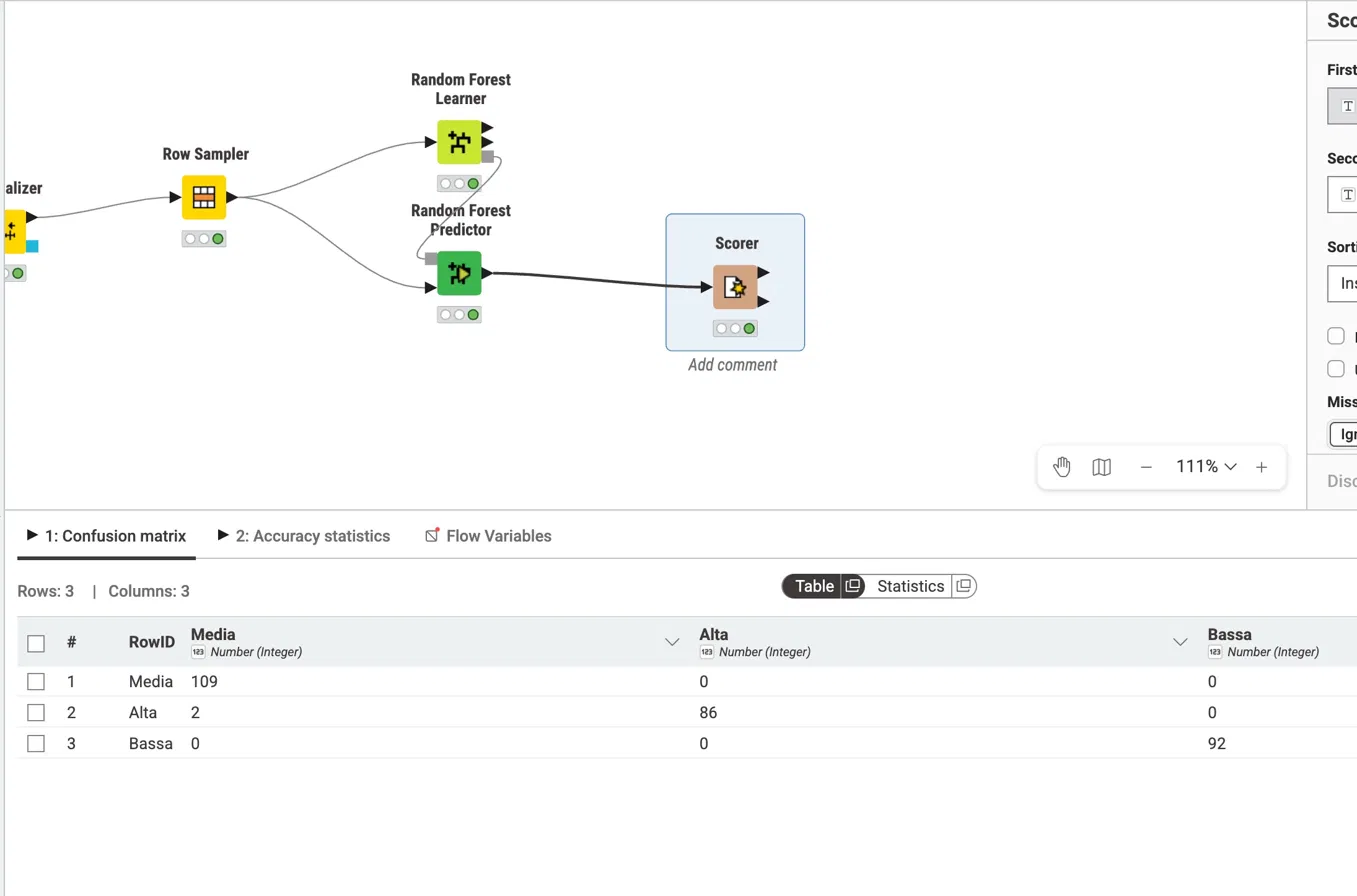
\includegraphics[width=0.85\textwidth]{knime_confusion_matrix.png}
  \caption{Matrice di confusione prodotta dallo Scorer KNIME. L'elevata
           accuracy (99,3\%) è dovuta al fatto che il Predictor valuta
           dati già visti in fase di training — limitazione del nodo
           \textit{Row Sampler} in KNIME~5. I risultati di riferimento
           sono quelli ottenuti in Python (Tabella~\ref{tab:risultati}).}
  \label{fig:knime_cm}
\end{figure}

% ══════════════════════════════════════════════════════════════
\section{Risultati e Valutazione}
% ══════════════════════════════════════════════════════════════

\subsection{Metriche di valutazione}

Per la valutazione dei modelli sono state usate le metriche standard della
classificazione multiclasse.

L'\textbf{accuracy} misura la proporzione di predizioni corrette:
$\text{Acc} = \frac{TP + TN}{TP + TN + FP + FN}$

\textbf{Precision}, \textbf{Recall} e \textbf{F1-score} vengono calcolate per
ogni classe e poi mediate (\textit{macro average}):
\begin{align}
  \text{Precision} &= \frac{TP}{TP + FP} \\[4pt]
  \text{Recall}    &= \frac{TP}{TP + FN} \\[4pt]
  F_1              &= 2 \cdot \frac{\text{Precision} \cdot \text{Recall}}
                         {\text{Precision} + \text{Recall}}
\end{align}

\subsection{Confronto tra modelli}

\begin{table}[H]
\centering
\caption{Risultati comparativi dei tre modelli su training (CV) e test set}
\rowcolors{2}{sfondotab}{white}
\begin{tabular}{lcccc}
  \toprule
  \textbf{Modello} & \textbf{Acc.\ test} & \textbf{CV media} & \textbf{CV std}
  & \textbf{F1 macro (test)} \\
  \midrule
  Decision Tree  & 0,598 & 0,564 & 0,104 & 0,597 \\
  Random Forest  & 0,577 & \textbf{0,622} & \textbf{0,084} & 0,581 \\
  Naive Bayes    & 0,556 & 0,561 & 0,059 & 0,554 \\
  \bottomrule
\end{tabular}
\label{tab:risultati}
\end{table}

\begin{figure}[H]
  \centering
  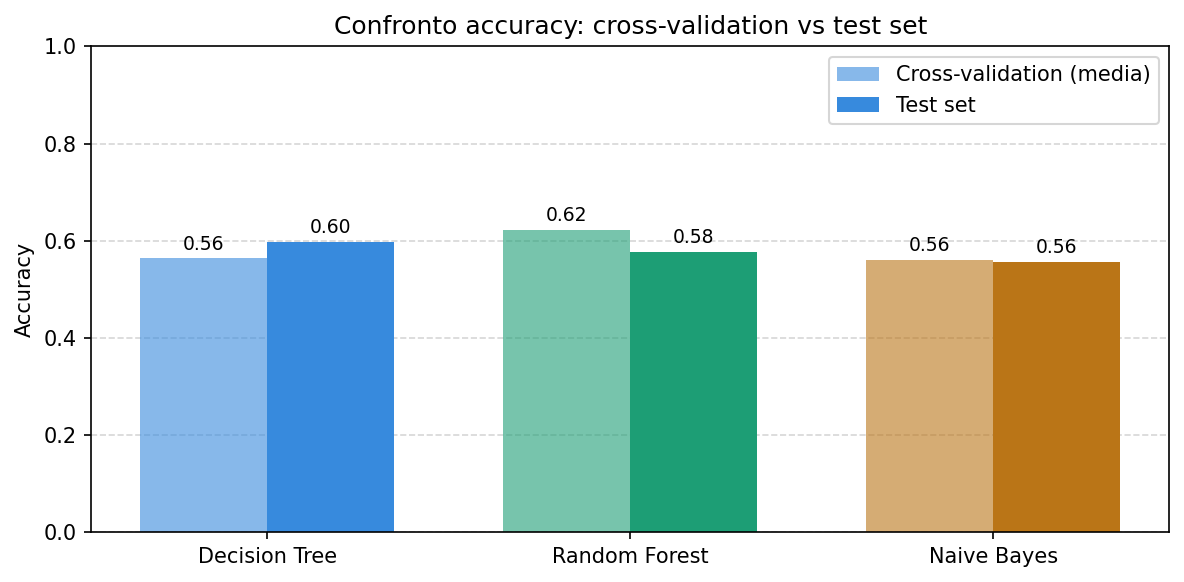
\includegraphics[width=0.95\textwidth]{grafico_accuracy.png}
  \caption{Confronto tra accuracy media in cross-validation e accuracy sul
           test set per i tre modelli.}
  \label{fig:accuracy}
\end{figure}

I risultati sono \textbf{significativi}: in un problema di classificazione a
tre classi equiprobabili, un classificatore casuale raggiungerebbe un'accuracy
del 33\%. I modelli addestrati raggiungono valori compresi tra il 55\% e il
60\%, raddoppiando di fatto la performance di una strategia casuale.

È importante notare la divergenza tra CV e test set per il Decision Tree
(0,564 vs 0,598): questo comportamento è tipico di un modello con varianza
elevata, che performa diversamente a seconda del sottoinsieme di dati su cui
viene valutato. La Random Forest mostra invece la \textbf{CV più alta e la
deviazione standard più bassa} (0,084), indicando maggiore stabilità e
migliore capacità di generalizzazione, proprietà attese dall'ensemble learning.

\subsection{Analisi per classe}

\begin{table}[H]
\centering
\caption{Precision, Recall e F1-score per classe — Random Forest}
\rowcolors{2}{sfondotab}{white}
\begin{tabular}{lccc}
  \toprule
  \textbf{Classe} & \textbf{Precision} & \textbf{Recall} & \textbf{F1-score} \\
  \midrule
  Alta  & 0,633 & 0,655 & 0,644 \\
  Bassa & 0,583 & 0,677 & 0,627 \\
  Media & 0,516 & 0,432 & 0,471 \\
  \bottomrule
\end{tabular}
\label{tab:perclasse}
\end{table}

La classe \textbf{Media} è la più difficile da classificare per tutti i modelli,
con F1-score sistematicamente inferiore alle altre due classi. Questo risultato
è interpretabile: le offerte ``medie'' sono quelle in cui il Dottore si comporta
in modo meno prevedibile, variando il suo ratio in un intervallo ampio a seconda
di fattori contestuali (regione del concorrente, dinamiche narrative della
puntata, valore dei singoli pacchi rimasti) che non sono pienamente catturati
dalle feature numeriche disponibili. Le classi \textbf{Alta} e \textbf{Bassa},
al contrario, corrispondono a comportamenti più stereotipati e riconoscibili.

\begin{figure}[H]
  \centering
  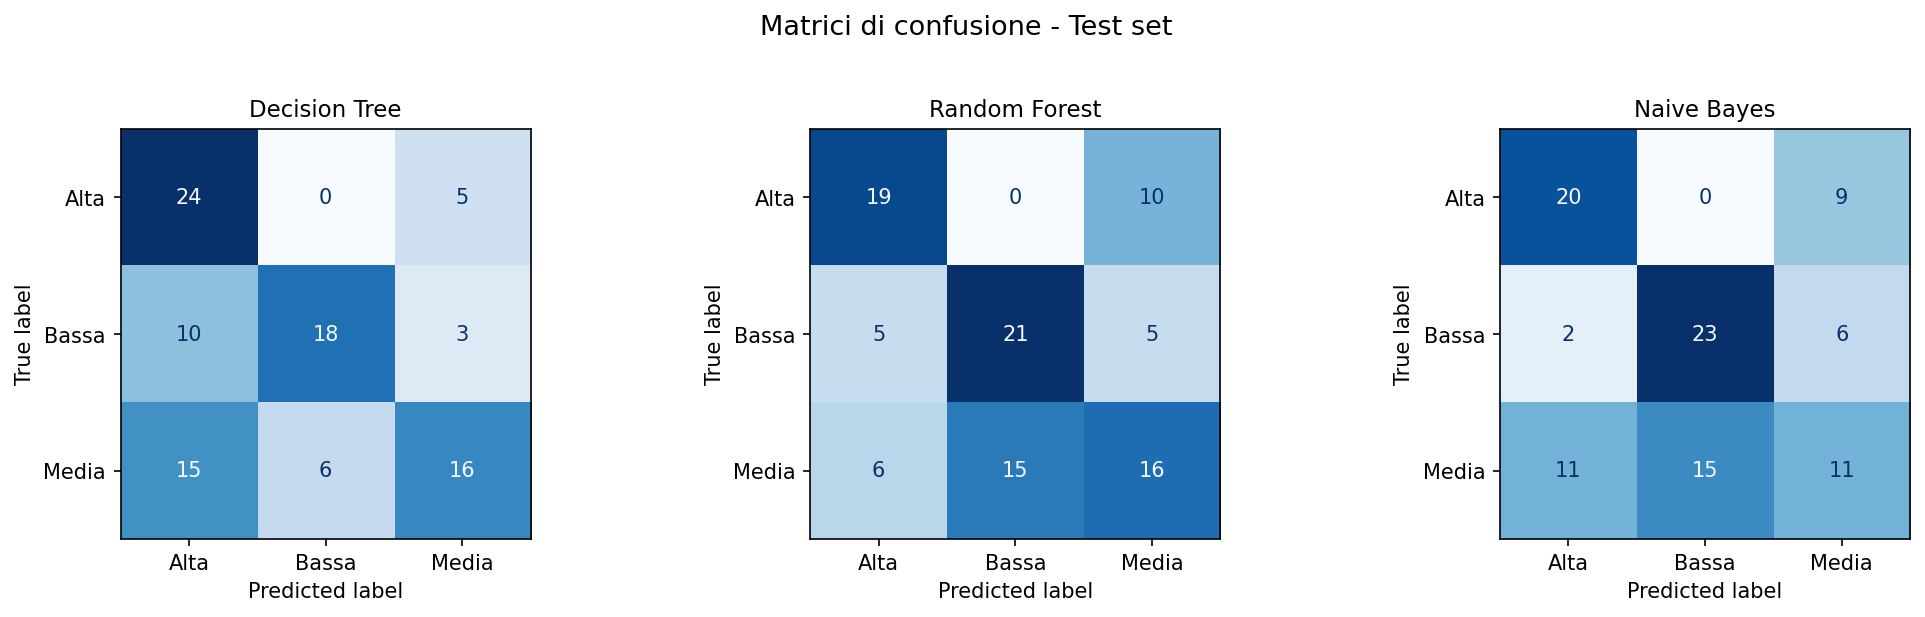
\includegraphics[width=\textwidth]{matrici_confusione.png}
  \caption{Matrici di confusione per i tre modelli sul test set.
           I valori sulla diagonale principale rappresentano le predizioni
           corrette.}
  \label{fig:confusione}
\end{figure}

\subsection{Feature importance}

\begin{figure}[H]
  \centering
  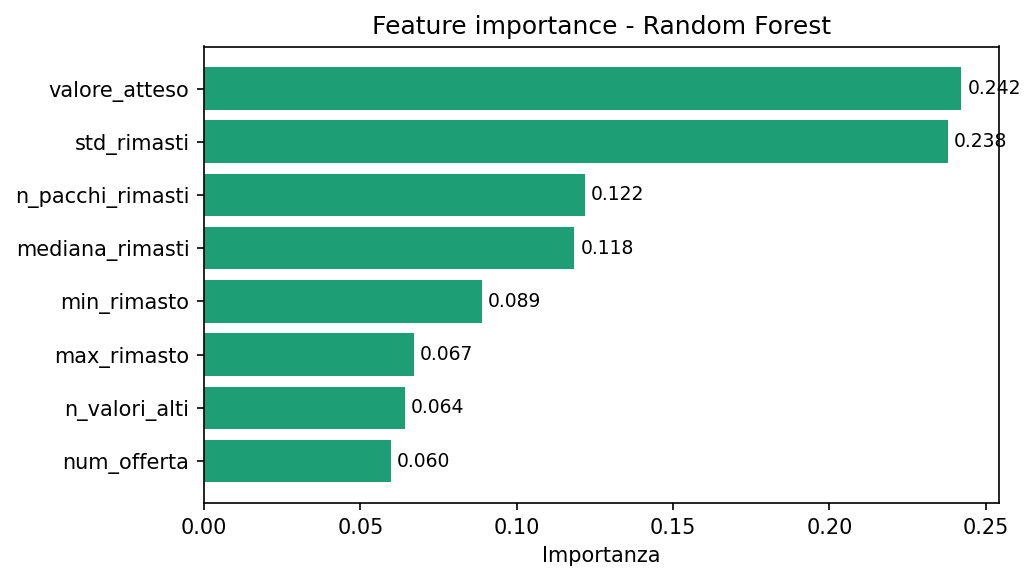
\includegraphics[width=0.85\textwidth]{feature_importance.png}
  \caption{Importanza delle feature secondo la Random Forest, misurata come
           riduzione media dell'impurità di Gini.}
  \label{fig:importance}
\end{figure}

Il grafico di feature importance rivela una gerarchia informativa chiara.
Il \textbf{valore atteso} è di gran lunga la feature più predittiva (importanza
$\approx 0{,}28$): è logico, perché è il denominatore del ratio e quindi la
quantità che il Dottore deve conoscere per formulare qualsiasi offerta. A seguire
troviamo \textbf{max\_rimasto} e \textbf{std\_rimasti}, che catturano il
``rischio'' per la produzione: quando è rimasto un pacco da 300.000~€, il
Dottore ha tutto l'interesse a formulare un'offerta che spinga il concorrente a
vendere. Il \textbf{numero di pacchi rimasti} e il \textbf{turno di offerta}
completano il quadro, confermando il pattern temporale emerso nell'analisi
esplorativa.

% ══════════════════════════════════════════════════════════════
\section{Interpretazione: quanto trattiene il Dottore?}
% ══════════════════════════════════════════════════════════════

Il vero contributo di questo progetto non è tanto tecnico quanto
\textbf{narrativo}: le predizioni del modello permettono di rispondere
alla domanda con cui si è aperto questo elaborato.

\subsection{Quanto è distante l'offerta dalla matematica?}

Nell'intera stagione analizzata, la media dell'offerta è stata di \textbf{30.770~€}
a fronte di un valore atteso medio di \textbf{41.007~€}. Il Dottore ha quindi
trattenuto in media \textbf{10.237~€ per offerta} — circa il 25\% del valore
matematicamente atteso.

Il comportamento non è però uniforme. Gli esempi reali estratti dal test set
illustrano i due estremi:

\begin{tcolorbox}[colback=rossoat!6, colframe=rossoat!60!black,
  fonttitle=\bfseries\small, title=Offerta classificata come BASSA --- esempio reale]
\small
\textbf{Data}: 20 aprile 2024 \quad \textbf{Turno}: 3\textsuperscript{a} offerta\\
\textbf{Pacchi rimasti}: 7 \quad \textbf{Valore atteso}: 57.305~€\\
\textbf{Offerta del Dottore}: 38.000~€\\
\textit{Trattenuto: \textbf{19.305~€} (34\% del valore atteso)}\\[4pt]
Il modello ha correttamente classificato questa offerta come \textit{Bassa},
riconoscendo che il Dottore stava offrendo meno di due terzi del valore
matematicamente atteso in un momento di alta pressione (terza offerta,
molti pacchi ad alto valore ancora in gioco).
\end{tcolorbox}

\vspace{0.5cm}

\begin{tcolorbox}[colback=verdeat!6, colframe=verdeat!60!black,
  fonttitle=\bfseries\small, title=Offerta classificata come ALTA --- esempio reale]
\small
\textbf{Data}: 5 marzo 2024 \quad \textbf{Turno}: 6\textsuperscript{a} offerta\\
\textbf{Pacchi rimasti}: 3 \quad \textbf{Valore atteso}: 40.333~€\\
\textbf{Offerta del Dottore}: 60.000~€\\
\textit{Ratio: \textbf{1,49} --- il Dottore ha offerto il 49\% in più del valore atteso}\\[4pt]
In questo caso il modello ha classificato correttamente l'offerta come \textit{Alta}.
Con soli 3 pacchi rimasti e una struttura di valori molto favorevole, la
produzione ha preferito ``comprare'' la certezza evitando il rischio di pagare
il massimo.
\end{tcolorbox}

\subsection{Implicazioni pratiche}

Il modello non ha valore predittivo in senso assoluto (un concorrente non può
attendere la risposta dell'algoritmo prima di decidere), ma ha un valore
\textbf{analitico} e \textbf{conoscitivo} fondamentale: dimostra che le offerte
del Dottore seguono una logica \textit{apprendibile}, cioè che esistono pattern
statisticamente riconoscibili nel suo comportamento.

In particolare:

\begin{itemize}
  \item \textbf{Il Dottore non è casuale.} Se le offerte fossero formulate
        senza logica, nessun modello ML potrebbe superare significativamente il
        33\% di accuracy su un problema a tre classi. Il fatto che i nostri
        modelli raggiungano il 56--60\% è la prova che un pattern esiste.
  \item \textbf{Il Dottore è più aggressivo a metà partita.} Il ratio scende
        al minimo al terzo turno (0,729) e aumenta nelle fasi finali
        (0,893), coerentemente con una strategia volta a sfruttare il momento
        di massima incertezza psicologica per il concorrente.
  \item \textbf{I premi alti influenzano l'offerta più dei premi bassi.}
        La feature importance indica che \texttt{max\_rimasto} e \texttt{std\_rimasti}
        sono tra le variabili più predittive, confermando che il Dottore calibra
        l'offerta soprattutto in funzione del ``rischio'' rappresentato dai
        pacchi ad alto valore ancora in gioco.
\end{itemize}

% ══════════════════════════════════════════════════════════════
\section{Regressione: stima dell'offerta in euro}
% ══════════════════════════════════════════════════════════════

La classificazione in tre classi risponde alla domanda
\textit{``il Dottore è avaro, nella norma o generoso?''}
ma non fornisce una stima monetaria precisa. Per rispondere direttamente
alla domanda \textit{``quanto offrirà il Dottore in euro?''} si è
implementato un secondo modello: una \textbf{Random Forest Regressor}
che predice il \textbf{ratio offerta/valore atteso} come valore
continuo. Moltiplicando il ratio predetto per il valore atteso dei
premi rimasti si ottiene la \textbf{stima dell'offerta in euro}.

\subsection{Impostazione del modello}

Il modello di regressione utilizza le stesse 8 feature e lo stesso
split train/test (75\%/25\%, seed~42) della classificazione.
Il target non è più la classe categorica ma il \textbf{ratio continuo}
$\hat{r} \in \mathbb{R}^+$, e la stima dell'offerta viene calcolata come:

\begin{equation}
  \hat{O} = \hat{r} \times \mathbb{E}[\text{premi rimasti}]
\end{equation}

Le metriche di valutazione usate per la regressione sono:

\begin{itemize}
  \item \textbf{MAE} (\textit{Mean Absolute Error}): errore medio assoluto,
        misura di quanto la stima si discosta in media dalla realtà;
  \item \textbf{RMSE} (\textit{Root Mean Squared Error}): penalizza
        maggiormente gli errori grandi;
  \item \textbf{R²} (\textit{coefficiente di determinazione}): misura la
        proporzione di varianza spiegata dal modello (1 = perfetto, 0 = casuale).
\end{itemize}

\subsection{Risultati}

\begin{table}[H]
\centering
\caption{Metriche del modello di regressione (Random Forest, test set)}
\rowcolors{2}{sfondotab}{white}
\begin{tabular}{lcc}
  \toprule
  \textbf{Metrica} & \textbf{Sul ratio} & \textbf{Sull'offerta in €} \\
  \midrule
  MAE  & 0,0893 (~8,9\% dal ratio reale) & 3.163~€ \\
  RMSE & 0,1204 & 4.494~€ \\
  R²   & 0,514  & --- \\
  CV MAE (10-fold) & 0,1067 ± 0,0158 & --- \\
  \bottomrule
\end{tabular}
\label{tab:regressione}
\end{table}

Il modello spiega il \textbf{51,4\% della varianza} delle offerte del
Dottore con un errore medio di soli \textbf{3.163~€} — un risultato
notevole considerando che le offerte spaziano da poche centinaia a
centinaia di migliaia di euro.

\begin{figure}[H]
  \centering
  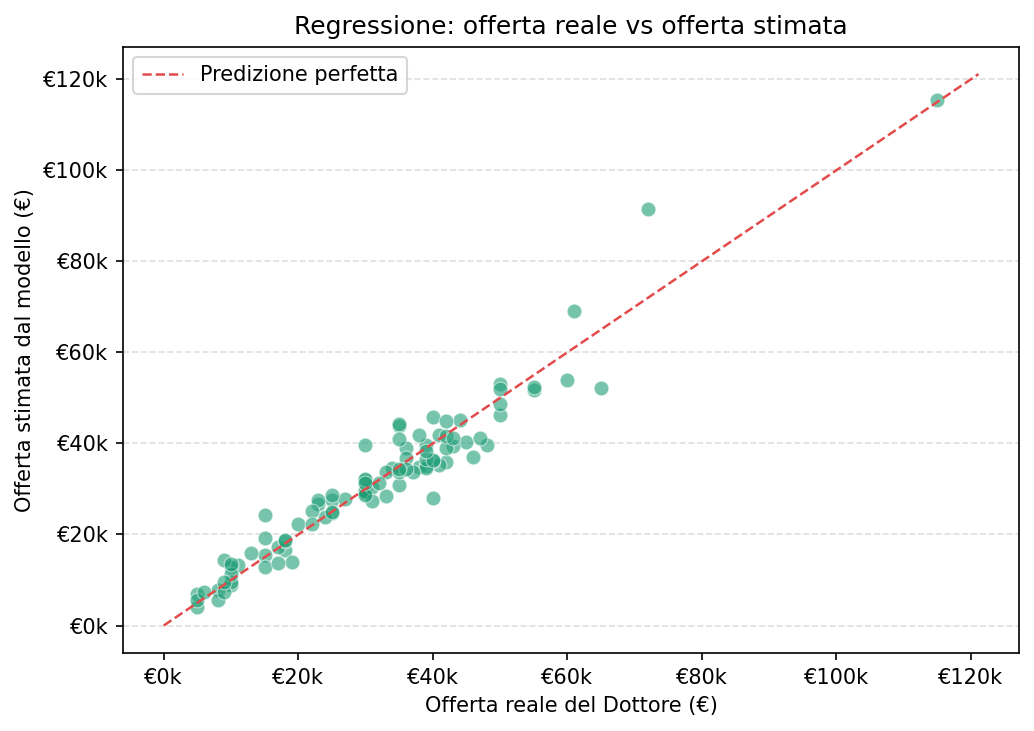
\includegraphics[width=0.85\textwidth]{regressione_scatter.png}
  \caption{Offerta reale del Dottore vs offerta stimata dal modello di
           regressione. I punti sulla linea tratteggiata rossa
           rappresentano predizioni perfette.}
  \label{fig:scatter}
\end{figure}

\begin{figure}[H]
  \centering
  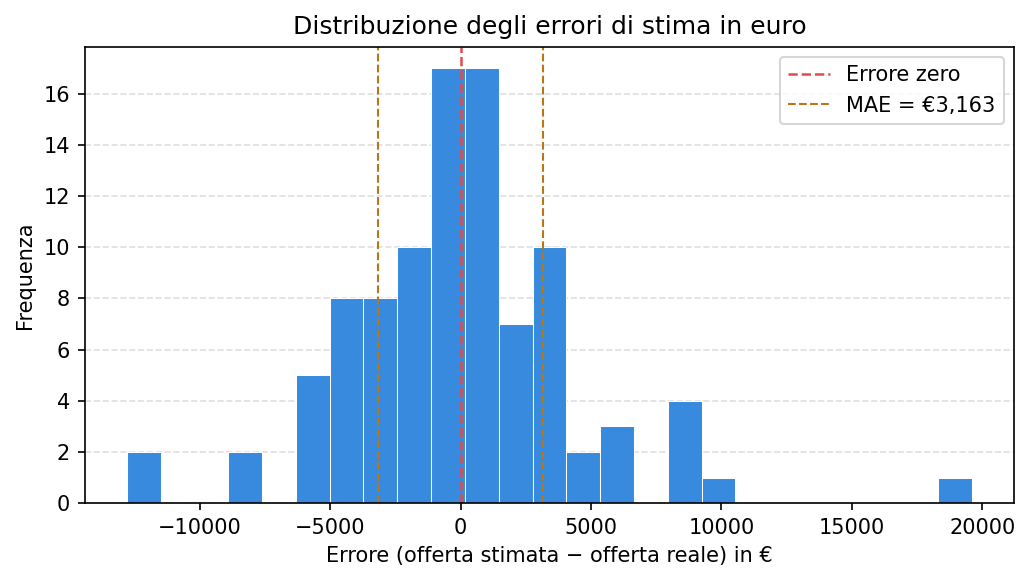
\includegraphics[width=0.85\textwidth]{regressione_errori.png}
  \caption{Distribuzione degli errori di stima in euro
           (offerta stimata $-$ offerta reale). La distribuzione è
           centrata attorno allo zero, senza bias sistematici evidenti.
           Le linee tratteggiate arancioni indicano il MAE (±3.163~€).}
  \label{fig:errori}
\end{figure}

\subsection{Esempi concreti}

La Tabella~\ref{tab:esempi_reg} mostra i casi in cui il modello ha
stimato l'offerta con maggiore precisione, dimostrando la capacità
concreta di quantificare il comportamento del Dottore.

\begin{table}[H]
\centering
\caption{I cinque casi con stima più accurata (test set)}
\rowcolors{2}{sfondotab}{white}
\begin{tabular}{cccccc}
  \toprule
  \textbf{Data} & \textbf{Turno} & \textbf{VA (€)} &
  \textbf{Offerta reale} & \textbf{Stima modello} & \textbf{Errore} \\
  \midrule
  05/05/2024 & 2\textsuperscript{o} & 10.250 & 8.000  & 7.891  & $-$109~€ \\
  15/04/2024 & 4\textsuperscript{o} & 17.167 & 17.000 & 17.148 & $+$148~€ \\
  20/05/2024 & 4\textsuperscript{o} & 35.136 & 25.000 & 24.849 & $-$151~€ \\
  17/02/2024 & 4\textsuperscript{o} & 26.214 & 24.000 & 23.826 & $-$174~€ \\
  10/05/2024 & 1\textsuperscript{o} & 50.450 & 42.000 & 41.684 & $-$316~€ \\
  \bottomrule
\end{tabular}
\label{tab:esempi_reg}
\end{table}

Il caso più accurato è emblematico: con un valore atteso di 10.250~€,
il Dottore ha offerto 8.000~€ e il modello ha stimato 7.891~€ —
un errore di soli \textbf{109~€}. Questo livello di precisione conferma
che le offerte seguono una logica strutturata che un algoritmo addestrato
su dati storici è in grado di riprodurre.

% ══════════════════════════════════════════════════════════════
\section{Conclusioni}
% ══════════════════════════════════════════════════════════════

Questo progetto ha dimostrato come le tecniche di \textbf{Machine Learning
supervisionato} possano essere applicate con successo a un dominio inatteso
come quello di un gioco televisivo, producendo risultati al tempo stesso
tecnicamente validi e di interesse divulgativo.

I tre classificatori addestrati (Decision Tree, Random Forest, Naive Bayes)
hanno raggiunto accuracy tra il 55\% e il 60\% su un problema a tre classi
con baseline casuale al 33\%, con la Random Forest che si è distinta per la
maggiore stabilità in cross-validation ($\mu = 0{,}622$, $\sigma = 0{,}084$).

Il modello di regressione ha ulteriormente affinato l'analisi, stimando
l'offerta del Dottore con un errore medio di \textbf{3.163~€} e un
R² di \textbf{0,514} — dimostrando che il comportamento del Dottore
non è solo classificabile ma direttamente quantificabile in euro.

L'analisi delle feature importance ha evidenziato che il \textbf{valore atteso},
il \textbf{massimo rimasto} e la \textbf{deviazione standard} dei premi in gioco
sono i fattori che più determinano il comportamento del Dottore, confermando
l'ipotesi che le offerte seguano una logica di \textbf{minimizzazione del
rischio} per la produzione.

\paragraph{Limiti del lavoro.}
Il principale limite è la \textbf{dimensione del dataset}: 386 offerte sono
sufficienti per un progetto didattico, ma insufficienti per addestrare modelli
ad alta capacità come le reti neurali. L'ampliamento del dataset a più stagioni
di gioco potrebbe migliorare significativamente le performance. Ulteriori
feature potenzialmente rilevanti — come la \textbf{regione di provenienza} del
concorrente o il \textbf{mese} della puntata — non erano disponibili nel
dataset utilizzato.

\paragraph{Sviluppi futuri.}
Alcune direzioni di ricerca meritano approfondimento:
\begin{itemize}
  \item Estendere il dataset alle stagioni precedenti per aumentare la potenza
        statistica;
  \item Esplorare tecniche di \textbf{spiegabilità} (SHAP values, LIME) per
        motivare le singole predizioni in modo interpretabile;
  \item Analizzare eventuali \textbf{differenze regionali} nel comportamento
        del Dottore, aspetto particolarmente discusso nel dibattito pubblico.
\end{itemize}

\paragraph{Considerazione finale.}
I risultati di questo progetto sono coerenti con le analisi statistiche
pubblicate da altri ricercatori sullo stesso programma: le offerte del Dottore
non sono casuali e seguono schemi riconoscibili. Il Machine Learning aggiunge
a questa osservazione una dimensione predittiva concreta: non solo il Dottore
\textit{si comporta} in modo sistematico, ma quel comportamento è
\textit{apprendibile} e \textit{quantificabile in euro} da un algoritmo
addestrato su dati storici.

% ══════════════════════════════════════════════════════════════
\section*{Extra — Il Dottore Artificiale: un gioco da terminale}
\addcontentsline{toc}{section}{Extra — Il Dottore Artificiale: un gioco da terminale}
% ══════════════════════════════════════════════════════════════

Il modello di regressione non è solo un numero su una tabella.
Per dimostrarlo in modo concreto e divertente, è stato realizzato
\textbf{gioca.py}: uno script Python che simula una vera puntata di
\textit{Affari Tuoi} da terminale, usando il modello addestrato come
cervello del Dottore.

L'idea di fondo è semplice ma potente: se il modello ha davvero imparato
la logica del Dottore, dovrebbe essere in grado di replicarla in tempo
reale su una partita mai vista. Non su dati storici, non su un test set
— ma su una partita generata casualmente, pacco per pacco, proprio come
accade in televisione ogni sera.

\paragraph{Come funziona.}
All'avvio, i 21 premi vengono distribuiti casualmente nei pacchi.
Il giocatore sceglie il proprio pacco e, turno dopo turno, apre quelli
degli altri concorrenti. Al termine di ogni turno il modello calcola
le stesse feature usate in fase di addestramento — valore atteso,
massimo rimasto, deviazione standard, numero di premi alti ancora in
gioco — e stima quanto offrirebbe il Dottore reale in quella situazione.
L'offerta viene presentata insieme al ratio predetto, così il giocatore
può vedere non solo il numero in euro ma anche il ragionamento dietro:
\textit{``il Dottore sta offrendo il 74\% del valore atteso — è
un'offerta nella norma''}.

\paragraph{Perché è significativo.}
Un modello che funziona solo su dati di test potrebbe aver semplicemente
memorizzato dei pattern. Un modello che genera offerte plausibili su
partite casuali, mai viste durante il training, dimostra di aver
generalizzato la logica sottostante. Il gioco è quindi il banco di prova
più onesto del progetto: ogni partita è un esperimento nuovo.

\paragraph{Come eseguirlo.}
Il file \texttt{gioca.py} si trova nella cartella \texttt{game/}
del repository. Prima di giocare è necessario eseguire almeno una volta
\texttt{affari\_tuoi\_ml.py}, che genera il file
\texttt{modello\_dottore.pkl} contenente il modello serializzato.
Poi basta lanciare:

\begin{lstlisting}[language=bash, caption={Avvio del gioco da terminale}]
cd game
python3 gioca.py
\end{lstlisting}

Il gioco gira interamente nel terminale, con colori e formattazione
che rendono leggibile il tabellone dei pacchi, i premi rimasti divisi
per fascia di valore e l'offerta del Dottore con il relativo ratio.
Alla fine di ogni partita viene mostrato il confronto tra l'offerta
accettata e il valore reale del pacco, permettendo al giocatore di
valutare se la decisione è stata corretta dal punto di vista matematico.

% ══════════════════════════════════════════════════════════════
\begin{thebibliography}{9}

\bibitem{mitchell1997}
  T.M. Mitchell,
  \textit{Machine Learning},
  McGraw-Hill, 1997.

\bibitem{breiman1984}
  L. Breiman, J. Friedman, C.J. Stone, R.A. Olshen,
  \textit{Classification and Regression Trees},
  Chapman \& Hall/CRC, 1984.

\bibitem{breiman2001}
  L. Breiman,
  ``Random Forests'',
  \textit{Machine Learning}, vol.~45, n.~1, pp.~5--32, 2001.

\bibitem{scikit}
  F. Pedregosa et al.,
  ``Scikit-learn: Machine Learning in Python'',
  \textit{Journal of Machine Learning Research}, vol.~12, pp.~2825--2830, 2011.

\bibitem{luzo7}
  luzo7,
  \textit{Affari Tuoi Dataset},
  GitHub, 2024.
  \url{https://github.com/luzo7/affari-tuoi}

\bibitem{parenti}
  P. Parenti,
  \textit{Affari Tuoi Fairness Analysis},
  GitHub, 2024.
  \url{https://github.com/PietroParenti/affari-tuoi-fairness}

\end{thebibliography}

\end{document}
